\graphicspath{{chapters/6.Chapter_4/figures/}}

\begin{savequote}[75mm]
In biology, nothing is clear, everything is too complicated, everything is a mess, 
and just when you think you understand something, you peel off a layer and find 
deeper complications beneath. Nature is anything but simple.
	\qauthor{- Richard Preston: The Hot Zone}
\end{savequote}

\chapter{RNAi in \textit{P. bursaria}}

\section{Introduction}

\subsection{RNAi}

Post-transcriptional gene silencing (PTGS) is a highly useful experimental technique
in reverse genetic analyses.
The most widely used PTGS experimental method is that of RNA-mediated inteference (RNAi)
of gene expression \citep{Fire1998}. It has extensively used in the
study of model eukaryotic organisms \citep{Morf2013,Batista2011,Matthew2004,Ketting2011,Chang2012}.

RNAi covers a whole set of evolutionarily conserved systems across the eukaryotes 
with various mechanisms of action in which the expression of particular transcripts
are regulated via several classes of transcribed small non-coding RNA (ncRNA)
such as short-interfering (siRNA), micro (miRNA) and Piwi-interacting (piRNAs) \citep{Carthew2009}.

These systems likely originated as a form of defence against
viruses and transposons \citep{Waterhouse2001,Buchon2006}
and were present in some form in the last universal eukaryotic
ancestor (LECA) \citep{Cerutti2006,Shabalina2008}.  Many eukaryotes
utilise these small RNA-mediated gene silencing pathways
in the regulation of their own cell expression patterns \citep{Wu2008}.
Despite its ancestral nature there has been considerable diversification
of both this process, its function and mechanism \citep{Ketting2011}.
Indeed, even within the same organism, different points of the life cycle
may use different RNAi systems \citep{Flemr2013}.


Generally RNAi pathways involve the generation of 21-28nt siRNAs
from some form of RNA precursor such as dsRNA (although ssRNA systems exist)
via the function of the RNAase III Dicer \citep{Bernstein2001} or a related protein. 
These short RNAs are then bound by Argonaute proteins which act alone or as part
of a complex to silence the expression of sequences homologous to the siRNA \citep{Ketting2011}.
This silencing isn't just limited to the post-transcriptional endonucleocytic degradation of 
mRNA transcripts but can also involve transcriptional inhibition and
DNA elimination \citep{Marker2014}.
The one unifying element of all discovered RNAi pathways is that
of the central role argonaute (AGO) proteins play \citep{Ketting2011}.
They are formed of two subclasses: the Ago and Piwi subfamilies \citep{Peters2007}
with a range of functions and complex-forming behaviours
\citep{Ender2010}.
The magnitude of the silencing response is occasionally amplified by the generation
of more copies of the trigger dsRNA by RNA-dependent RNA polyermases (RdRPs) \citep{Arp2007}.
On the other hand RdRPs can also sometimes directly generate the siRNAs \citep{Aoki2007,Ketting2011}.
The last universal eukaryotic ancestor (LECA) likely contained 
at least one Ago and Piwi family Argonaute protein, a Dicer and an RdRP \citep{Cerutti2006}.

The other main form of RNAi system present in eukaryotes is that of 
miRNA based systems.  These are differentiated
by miRNAs being encoded by dedicated genes and displaying partial
complementarity to their targets whereas siRNAs are generated from exogenous
dsRNAs (i.e. environmental dsRNA from viral infection or phagocytosed bacteria \citep{Whangbo2008})
or transgenes as described above and involve full or near full complementarity \citep{Shabalina2008}.

On top of this, there are piRNA based systems, which are involved in germline based transposon 
silencing \citep{Iwasaki2015}, and the ciliate specific scan RNA (scnRNA) system.
This is involved in the elimination of internal eliminated sequences (IESs) during
macronuclear (MAC) regeneration \citep{Mochizuki2004,Kiefer2013}.


Experimentally, the existence and function of these systems
permits a researcher to introduce dsRNA homologous to an RNA transcript of interest
and trigger targeted cell-wide RNAi of that transcript.
Unforunately, there also several problems with RNAi as a general method.
Many organisms lack active RNAi systems (although such systems can occasionally
be induced \citep{Alibu2005}).
On top of this, RNAi requires accurate sequence data to design the precursors
therefore necessitates some form of sequencing. 
The main difficulty, however, is that of off-target effects.
These are caused when a provided sRNA precursor induces RNAi
in more than just the target transcript.  These
can lead to enigmatic phenotypic outcomes that 
are then falsely attributed to the initial target.
Avoidance of off-target effects 
requires a complete genome and/or transcriptome
to check a prospective siRNA against during the design
stage.  This further increases the epistemological
burden of attempting RNAi in a novel system.

Finally, RNAi does not necessarily induce total silencing
of a given transcript and low-levels of transcription may still occur.
This, conceivably, can be sufficient to maintain the non-knock down phenotype.
This allows a researcher to falsely conclude a non-relationship between
a given transcript and phenotype.

\subsection{RNAi in \textit{Paramecium}}

In addition to the ciliate specific scnRNA system 
siRNA based pathways have been discovered in the two principal
ciliate model organisms: \textit{Tetrahymena thermophila} \citep{Collins2006,Yao2005}
and \textit{Paramecium tetaurelia} \citep{Galvani2001,Galvani2002}. 
There are two established methods for inducing RNAi in \textit{Paramecium tetaurelia}:
microinjection and transformation of the MAC with high-copy transgenes lacking 3' untranslated
region (UTR) \citep{Galvani2001} and the introduction of dsRNA by either
microinjection or feeding using transformed dsRNA expressing bacteria 
\citep{Galvani2002}.

In the transgene pathway, the 3' truncation leads to the production of aberrant
sense and antisense transcripts \citep{Galvani2001,Marker2010,Beisson2010b}.
Based on the identified required components (see \cref{tab:marker_components}), 
aberrant transcripts
are processed by a Dicer protein (Dcr1) \citep{Lepere2009} and
a putative RdRP complex formed of an RdRP (Rdr2) and a nucleotidyl
transferase (Cid2) \citep{Marker2014} into 23nt siRNA \citep{Lepere2009}. 
A putatively non-catytic 
RdRP (Rdr3) also plays an undefined role in the generation
of primary (\(1^{\circ}\)) siRNAs from transgene pre-cursors \citep{Marker2010,Marker2014}.
Finally, two Argonaute Piwi proteins (Ptiwi13 and Ptiwi14) \citep{Bouhouche2011} 
are involved in targeting post-transcriptional silencing via mRNA
cleavage \citep{Bouhouche2011,Marker2014}.


Alternatively, the exogenous dsRNA pathway can be induced by either microinjection directly
into the MAC (for a transient 48 hour long silencing) or by continued feeding
with a bacterially experimentally modified to generate dsRNA.
Typically, this involves an \textit{E. coli} 
with an IPTG-inducible T7 polymerase and 
deficiency for RNAse III transformed with
a plasmid containing a T7 promoter and the sequence
homologous to the target transcript
\citep{Fire1998,Timmons2001,Galvani2002}.
Importantly, there is some evidence that this pathway also is activated at low
levels by ssRNA from normal food bacteria \citep{Carradec2015}.

\begin{table}
    \centering
    \begin{tabular}{|c|c|c|}
        \hline
        \textbf{Pathway} & \textbf{Component} & \textbf{Function} \\
        \hline
        transgene-induced siRNA & Rdr3 & RdRP \\
                                & Ptiwi14 & Piwi \\
        both pathways           & Rdr2 & RdRP \\
                                & Dcr1 & Dicer \\
                                & Ptiwi13 & Piwi \\
                                & Cid2 & Nucleotidyl transferase \\
        exogenous dsRNA-induced siRNA & Rdr1 & RdRP \\
                                      & Cid1 & Nucleotidyl transferase \\
                                      & Ptiwi12 & Piwi \\
                                      & Ptiwi15 & Piwi \\
                                      & Pds1 & Import of dsRNA? \\
        \hline
    \end{tabular}
    \caption[Summary of RNAi pathway components in \textit{P. tetaurelia}]{Summary
        of the components identified as necessary to the function of both
        primary siRNA RNAi pathways in \textit{P. tetaurelia} as identified
        by forward genetic screens in \citep{Marker2014}}
    \label{tab:marker_components}
\end{table}


Based on the components that have been identified as necessary
for the exogenous dsRNA pathway to function (see \cref{tab:marker_components}).  
RNA precursors are processed
by Dcr1 \citep{Lepere2009}, and then two hypothetical RdRC (Cid1-Rdr1, Cid2-Rdr2)
\citep{Marker2010,Marker2014} are involved in the generation of \(1^{\circ}\) 
siRNA.  
The second RdRC (or specifically Rdr2) is also involved in the generation
of low levels of secondary (\(2^{\circ}\)) siRNA which spread along the full length of
target mRNA (i.e. 3'-to-5' and 5'-to-3' transitivity) in primarily
antisense form \citep{Carradec2015}.  These \(2^{\circ}\) siRNAs don't
appear to play a significant role in silencing themselves (contrary to similar
systems in \textit{C. elegans} where they form the principal targetter of silencing 
\citep{Sijen2007,Pak2007}) \citep{Carradec2015}.
3 Piwis play a role in targeting silencing.  Ptiwi13 hypothetically
loads the \(1^{\circ}\) siRNA and targets cleavage of cytoplasmic mRNA \citep{Bouhouche2011},
while Ptiwi12 and Ptiwi15, based on their homology to nuclear Piwi proteins,
\citep{Marker2014,Carradec2015,Bouhouche2011} may be involved
with \(2^{\circ}\) siRNA communication with the MAC \citep{Carradec2015}.
One final protein is necessary for the function of feeding based dsRNA-induced
RNAi is an uncharacterised novel \textit{P. tetaurelia} complex protein (Pds1) \citep{Marker2014}.
It has been hypothesised that Pds1 may play a role in the export of RNA from 
the food vacuole \citep{Carradec2015}.  Therefore, theoretically
microinjected dsRNA should induce RNAi even in the absence of this protein
as the microinjection circumvents the need for Pds1 facilitated dsRNA import.


Many of these components are a product of the 3 whole genome duplication
events in the evolution of the \textit{Paramecium} clade \citep{McGrath2014}.
As \textit{P. bursaria} shares only the first \textit{Paramecium} clade whole
genome duplication event with \textit{P. tetaurelia} it is expected
it should contain the RNAi components identified as belonging to WGD1 (or have 
secondarily lost them) \citep{McGrath2014}.
This is believed to include a single RdRP gene, 6 Piwi genes, and 2 Dicer genes \citep{Marker2014}.

%siRNAs are made endogenously from an intergenic lopcus of unknown functions \citep{Marker2010,Marker2014}
%exogenous ssRNAmay protect against horizontal transfer of ss retroelements \citep{Carradec2015}

%Although the clustered regularly interspaced short palindromic repeat (CRISPR)/Cas
%system can be used to simplify gene editing or deactivation (CRISPRi).
%This system is not available in \textit{Paramecium}.

If it is possible to experimentally induce RNAi in \textit{P. bursaria} SW1 (from CCAP 1660/12 culture)
specific hypotheses as to the necessity of hypothetically important
endosymbiotic components can be tested. For example, what is the effect
on endosymbiosis of the inhibition of certain host-derived transporters.

Similarly, what components of core \textit{P. tetaurelia} RNAi pathways
can be identified 
in the \textit{P. bursaria} SW1 (see Chapter 4) and \textit{P. bursaria} Yad1g transcriptomes
(see Chapter 5)?  Does \textit{P. bursaria} express these components during
endosymbiosis?  If they don't is there evidence of them in the partial 
\textit{P. bursaria} SW1 genome (see Chapter 3)?


\subsection{RNAi ``cross-talk''}
Evidence has emerged of the role RNAi plays in numerous host-pathogen 
\citep{Nowara2010,LaMonte2012,Weiberg2013,Buck2014}
and host-symbiont \citep{Helber2011,Koch2013} relationships.
This has led some authors to suggest that siRNA and RNAi mechanisms 
can form communication systems between diverse organisms and even across
domains \citep{Liang2013,Knip2014,Weiberg2015}.


The evidence of natural food bacteria ssRNA induced RNAi ``cross-talk''
in \textit{P. tetaurelia} \citep{Carradec2015} implicates
that this process may also take place in \textit{P. bursaria}.
In addition to also being a serial phagotroph \textit{P. bursaria}
acts as a host to numerous bacterial and green algal endosymbionts.
Therefore, it is not inconceivable that such a mechanism of 
cross-talk many play role in these endosymbioses.


Therefore, it may be informative to investigate the quantity and targets of
potential cross-talk between host and endosymbiont in terms of 
``collisions''  i.e. matching 23nt RNA strings between host and endosymbiont
transcripts bins.   Contextualising these values 
across the diversity of the tree of life is important.
``Collision'' levels have implications for the regulation and expression of exogenous dsRNA
RNAi pathways by the host. 
%While a \textit{Paramecium} virus is yet to be discovered there
%are evidence of the association of \textit{Paramecium bursaria-Chlorella} Viruses
%with the system therefore, it is not inconceivable that these may play some role.  


\section{Aims}

The goal of this chapter is to investigate both the practical and
theoretical utility of RNAi systems in \textit{P. bursaria}. 
Specifically:
\begin{itemize}
    \item Is \textit{P. bursaria} capable of microinjection or feeding based
        exogenous dsRNA siRNAi?
    \item What components, previously identified as necessary, for these pathways
        are present and expressed in \textit{P. bursaria}? 
    \item To what degree could potential RNAi ``cross-talk'' occur in \textit{P. bursaria}
        is this elevated compared to what might be faced in \textit{Paramecium} species
        without eukaryotic endosymbionts?
\end{itemize}


\section{Methods}

\subsection{RNAi constructs}

All RNAi methods were based on previously published protocols, specifically
\citep{Galvani2001,Galvani2002,Beisson2010}.

Six different constructs were created featuring genes whose knock-down
induces known phenotypes in \textit{P. tetaurelia} (see \cref{tab:rnai_vecs}).
All inserts were designed in the same manner, \textit{P. tetaurelia} sequences
were taken from the \textit{P. tetaurelia} genome. 
These were then BLASTN against the entire unbinned \textit{P. bursaria}-\textit{M. reissieri}
SW1-ZK transcriptome and designed based on the \textit{P. bursaria} sequence.
Each insert was cloned into an L4440 vector featuring two convergent T7 promoters
and an ampicillin resistance marker (shown in \cref{fig:vec_map}). 

\begin{figure}
    \includegraphics{l440_vector.pdf}
    \caption[L4440 RNAi Vector Map]{Schematic map of the L4440 vector used for the RNAi experiments. Site of the insert is highlighted in purple with the T7 promoters shown in green and the ampicillin marker in red. Figure was adapted from the unpublished Fire Lab \textit{C. Elegans} vector kit via Addgene (\url{https://www.addgene.org/1654/}).
    \label{fig:vec_map}
\end{figure}

\begin{table}
    \centering
    \resizebox{\textwidth}{!}{\begin{tabular}{|c|c|c|c|c|}
        \hline
    \textbf{Gene} & \textbf{Function} & \textbf{RNAi phenotype in}      & Vector Design & Reference \\
                  &                   & \textbf{\textit{P. tetaurelia}} &               &           \\
        \hline
        \textit{epi2} & Epiplasmin & ``Monstrous'' cells  & 500bp via \textit{Pst}I and \textit{Hind}III & \citep{Damaj2009} \\
        NSF & Membrane fusion factor & Lethal & 500bp via \textit{Pst}I and \textit{Hind}III & \citep{Galvani2002} \\
        pTMB.422c & Binding protein & Lethal & 500bp via \textit{Pst}I and \textit{Hind}III & \citep{Nowack2011} \\
        \textit{bug22} & Basal body/ciliary protein & Slow swimming and death & 313bp via \textit{Xba}I and \textit{Hind}III & \citep{Laligne2010} \\
        BBS7 & Ciliary ion transport & Fewer, shorter ciliar & 486bp via \textit{Xho}I and \textit{Hind}III & \citep{Valentine2012} \\
        PGM & PGM endonuclease & Post-autogamous cells unable to resume normal growth & 500bp via \textit{Pst}I and \textit{Hind}III & \citep{Baudry2009} \\
        \hline
\end{tabular}}
    \caption[Table of RNAi vectors and inserts used]{Details of RNAi vectors used in dsRNA experiments.  
    All constructs were cloned into a L4440 vector and used an Ampicillin resistance markers.}
    \label{tab:rnai_vecs}
\end{table}

\subsubsection{RNAi feeding}

For feeding experiments the vectors were transformed into \textit{E. coli} HT115-DE3.
This strain is deficient for RNAse III and features an IPTG inducible T7 polymerase
under the control of a Plac promoter. Method used was as described in \citep{Beisson2010}.
RT-PCR using standard methods was conducted on the transformed cultures
to confirm expression of the dsRNA.

Bacterial precultures were started using a single colony picked from an LB
plate containing \(50\mu gml^{-1}\) ampicillin and \(12.5\mu g ml^{-1}\) tetracyline.
This picked colony was grown overnight in LB medium with the same antibiotics.
The overnight culture was then diluted 50 fold and grown with shaking
at \(37\celsius\) up to an \(OD_{600}\) of 0.4 to 0.6. IPTG
was then added at a concentration of 0.4mM and shaken for 3 hours
at \(37\celsius\).  30ml of this culture was centrifuged for 2 minutes (3100 x g),
then the supernatant removed and the pellet washed twice in \textit{Paramecium}
growth medium. The pellet was resuspended in \textit{Paramecium} medium with 0.4mM IPTG,
\(100\mu g ml^{-1}\) ampicillin and adjusted to a final \(OD_{600}\) of 0.1.
\(1 \mu l\) of beta-sitosterol (at \(4mg ml^{-1}\) in ethanol) was added
to each 5ml of medium.

For the actual feeding, \(10ml\) \textit{P. bursaria} CCAP 1660/12 culture
were centrifuged at 800x g for 10 minutes and re-suspended in \(1ml\) of supernatant.
\(9ml\) of the induced bacterised media was then added.  The sample was
then incubated in a tissue culture flask at \(27\celsius\).
Feeding was repeated for each day of analysis. 

\subsubsection{RNAi microinjection}

Microinjection used the same protocol as described in \citep{Beisson2010b} 
but only tested the PGM construct.
Briefly, the circular plasmid is linearised using a unique restriction site,
and purified using phenol:ethanol extraction and a purification column.
It is then dissolved in \(H_{2}O\) at a mininmum concentration of 
\(5mg ml^{-1}\).
Cells were washed twice by picking with a micropippete in Dryl-BSA wells before
being placed into inidival droplets on a glass coverslip and covered in paraffin oil.
The coverslip was then placed onto a microscopy stage and a microinjector 
used under 10X mangification to inject linearised construct directly into the
macronucleus.

Microinjection controls were also conducted in which GFP was injected
into the MAC and the fluorescence observed.  Successful microinjection
would feature fluorescence localised to the MAC.

\subsection{Analysis of RNAi pathway}

\subsubsection{Survey for RNAi components in \textit{P. bursaria}}

Using the canonical seed sequences identified in \textit{P. tetaurelia}
by \citep{Marker2014} (see \cref{tab:rnai_seeds}) the entire assembled 
\textit{P. bursaria}-\textit{M. reisseri} SW1-ZK transcriptome predicted
ciliate encoding peptides and
\textit{P. bursaria}-\textit{C. variabilis} Yad1g1N transcriptome predicted 
ciliate encoding peptides with BLASTP and a minimum expectation
of \(1e^{-5}\).

Finally, if a component could not be identified in the transcriptomes
it was additionally searched for in the assembled \textit{P. bursaria}-\textit{M. reisseri} SW1-ZK
genomic contigs (over 500bp) using tBLASTx with a minimum expectation \(1e^{-5}\).
This would theoretically allow the identification of present but non-expressed components.

\begin{table}
    \centering
    \begin{tabular}{|c|c|c|}
        \hline
        \textbf{Gene} & \textbf{\textit{P. tetaurelia} Accession} & \textbf{Length} \\
        \hline
        Rdr1 & PTETG8500012001 & 4319 \\ 
        Rdr2 & GSPATG00036857001 & 4162 \\
        Rdr3 & GSPATG00006401001 & 3292 \\
        Cid1 & PTETG9100013001 & 1051 \\
        Cid2 & PTETG13400003001 & 1083 \\
        Pds1 & PTETG600032001 & 2084 \\
        Dcr1 & GSPATG00021751001 & 5394 \\
        Ptiwi12 & GSPATG00001709001 & 2315 \\
        Ptiwi13 & PTETG4800007001 & 2483 \\
        Ptiwi14 & PTETG16300003001 & 2428 \\
        Ptiwi15 & GSPATG00005370001 & 2315 \\
        \hline
    \end{tabular}
    \caption[RNAi pathway components from \citep{Marker2014}]{Table of
    the RNAi pathway components identified by \citep{Marker2014}. 
    Includes their ``canonical'' accession in the \textit{P. tetaurelia}
MAC genome.}
    \label{tab:rnai_seeds}
\end{table}

Additionally, the other sequenced \textit{Paramecium} genomes 
were searched using BLASTP via ParamediumDB \citep{Arnaiz2007,Arnaiz2011a}.
Specifically, \textit{P. caudatum} \citep{McGrath2014}, 
\textit{P. biaurelia}, \textit{P. primaurelia}, \textit{P. sexaurelia}
and \textit{P. multimicronucleatum}. Finally,  \textit{T. thermophila} \citep{Eisen2006}
and \textit{Oxytricha trifallax} \citep{Swart2013}
predicted proteins were searched to form outgroups during phylogenetic
analysis.

\subsubsection{Phylogenetic analysis of RNAi pathway}

Peptide sequences were aligned using MAFFT \citep{Katoh2002} and manually
masked in Seaview \citep{Gouy2010}.
Sequences that were too divergent to align were removed, or in the case
of the RdRPs: the alignment of Rdr1 and Rdr2 was split from that of Rdr3 to form
two separate alignments.  Similarly, sequences that were identical
to one another were removed at this stage. 

Substitution models were fitted using ProtTest3 on the basis of the Bayesian
Information Criterion (BIC) \citep{Darriba2011c}.
Phylogenies were then generated using RAxML with 1000 non-rapid bootstraps and MrBayes 
with 2 runs of 4 MCMCMC chains run for 2,000,000 generations or until convergence.
MCMC convergence was checked and burn-in determined using Tracer \citep{rambaut2007tracer}.
Sequences forming long branches were removed after inspection of these phylogenies
and the alignment, masking, model prediction and phylogeny generation steps
were repeated.

\subsubsection{Structural prediction and functional analysis}

The structure of Pds1  
was predicted from the \textit{P. tetaurelia} protein sequence 
(PTETP600032001) using RaptorX \citep{Kallberg2012}.
This prediction used default settings and was based on
a weighted combination of 
physicochemical features of the amino acids sequence, 
3D structural alignments, entropic modelling
and domain prediction \citep{Kallberg2012}.
The predicted structure was then plotted from the PDB
file using PyMOL \citep{DeLano2002}.

Using the PDB structure from RaptorX, functional prediction
was attempted using ProFunc \citep{Laskowski2005},
CombFunc \citep{Wass2012} and PredictProtein \citep{Rost2004} all
with default settings.

\subsection{dsRNA cross-talk analysis - ``eDicer''}

In order to investigate the prevalence of ``cross-talk'' between 
host and endosymbiont a tool to analyse short sequence collisions between two sets
of transcripts was created.  ``eDicer'' is built around 
the Jellyfish K-mer counter \citep{Marcais2011} 
and the K-mer Analysis Toolkit (KAT) \citep{ClavijoKAT}.  Using efficient
K-mer hashing it allows the identification of shared K-mers between
two sets of sequences.  As Dcr1 in \textit{P. tetaurelia} generates
23nt fragments, by identifying the number of shared 23-mers between
two datasets e.g. the set of host and endosymbiont transcripts 
we can identify the number of potential RNAi ``collisions'' or cross-talks
between the two species. 

For each comparison between a set of query transcripts and a reference
set of transcripts (endosymbiont transcripts in this case)
the following
values were calculated and tabulated:
\begin{itemize}
    \item Number of K-mers in the query, in other words the length of the query
        in K-mers (\(\frac{\sum^s_{n=1} len(x_{n})}{w}\)
        for a set containing \(s\) transcripts and a K-mer size of \(w\)).
    \item Number of unique K-mers in the query, the non-redundant length of 
        the query.
    \item Number of shared  K-mers (``collisions'') between query and subject bin.
    \item Number of unique shared K-mers betwee query and subject bin.
    \item Shared K-mers normalised by subject length in K-mers.
    \item Shared K-mers normalised by the subject length in unique K-mers.
    \item Shared unique K-mers normalised by subject length in K-mers.
    \item Shared unique K-mers normalised by the subject length in unique K-mers.
\end{itemize}

In order to contextualise the number of collisions between the 2
host and 2 endosymbiont transcript sets
I analysed the collisions between the two sets of endosymbiont transcripts 
with several other datasets.  

These datasets were composed of predicted or sequenced transcriptomes 
from the following groups: bacteria, 
archaea, eukaryotes, green algae, and the ciliates.
Sequences were selected to sample the breadth of the sequenced
diversity of each group as fully as possible.

Specifically, 3 ciliate transcript sets were used \textit{Paramecium tetaurelia}, 
\textit{Tetrahymena thermophila} and \textit{Oxytricha trifallax} along with
5 green algae \textit{Chlamydomonas reinhardtii}, \textit{Coccomyxa subellipsoidea}
C-169, \textit{Chlorella variabilis} NC64A, \textit{Micromonas pusilla} RCC299, and
\textit{Ostreococcus lucimarinus}.
The eukaryote dataset was composed of 58 transcript
sets (\cref{sec:edicer_genomes_euks}),
the bacterial 130 (\cref{sec:edicer_genome_bacteria}), and 
the archaea 89 (\cref{sec:edicer_archaea}).

Tabulated values were then analysed statistically
using standard python tools outlined in the methods chapter.

In the course of this work improvements made to KAT were submitted and merged
back into the core KAT development codebase (\url{https://github.com/TGAC/KAT})

\section{Results}

\subsection{Induction of RNAi}

There was a total failure to induce RNAi related phenotypes
in feeding experiments for any of the vectors. 
Despite observation for several days, continuous refeeding
with transformed \textit{E. coli} (and RT-PCR proof of dsRNA expression)
none of the \textit{P. bursaria} CCAP 1660/12 
cultures displayed any altered phenotypes as a consequence of feeding experiments. 


Microinjection was attempted using just the PGM and epi2 constructs due to
time constraints.
\textit{P. bursaria} tended to burst after a single injection attempt.
As a control, GFP was also attempted to be injected into the MAC.
Unfortunately, despite numerous attempts it was never possible
to observe fluorescence localised to the MAC. This suggests
microinjection was never successfully achieved. 

\subsection{RNAi pathway components}

\subsubsection{Dcr1}

A single Dcr1 orthologue was clearly identified in each of
the two \textit{P. bursaria} host transcriptomes.
Phylogenetic analysis (\cref{fig:dcr1}) recovered a phylogeny
matching the established ciliate taxonomy (\citep{Aury2006,Fokin2004,Swart2013}) 
with strong support for \textit{P. bursaria} as the the outgroup to the rest of 
the \textit{Paramecium} clade. 

\begin{figure}
    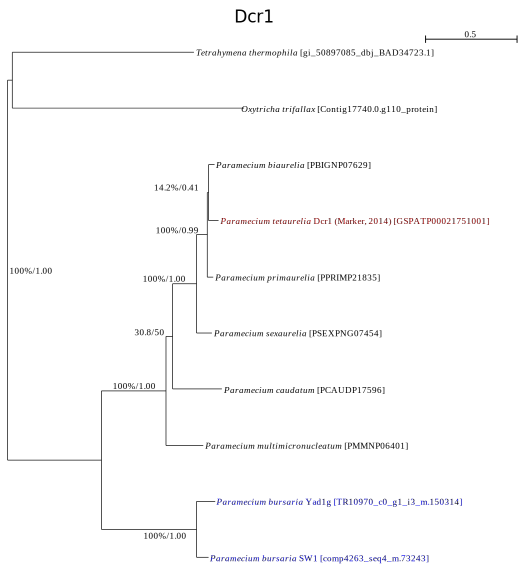
\includegraphics[width=\textwidth]{Dcr1.pdf}
    \caption[Dcr1 Phylogeny]{Dcr1 Phylogeny (1196 sites) inferred using RAxMl with
        LG+G+F and 1000 non-rapid bootstraps.  Bayesian PP 
        were inferred using MrBayes with 2 runs of 4 chains run for 2,000,000
        generations (5\% burnin) and the LG+G model.  \textit{P. bursaria} peptides
        are highlighted in blue whereas \textit{P. tetaurelia} components
    identified by \citep{Marker2014} are indicated in red.  Phylogeny
is largely consistent with established ciliate phylogenies.}
    \label{fig:dcr1}
\end{figure}


\subsubsection{Pds1}
There were no hits for Pds1 in any of the 3 \textit{P. bursaria} datasets 
(both transcriptomes and the genome).  
There were homologues in each of the other \textit{Paramecium} species
i.e. \textit{P. sexaurelia}, \textit{P. biaurelia}, \textit{P. primaurelia},
\textit{P. multimicronucleatum} and \textit{P. caudatum} but not
\textit{T. thermophila} or \textit{O. trifallax} (\cref{fig:pds1}).
\begin{figure}
    \includegraphics[width=\textwidth]{Psd1_tree.pdf}
    \caption[Pds1 Phylogeny]{Pds1 Phylogeny (424 sites) inferred
        using RAxML with VT+G+F and 1000 non-rapid bootstraps.  Bayesian
        PP were inferred with MrBayes (2 runs of 4 chains for 2,000,000 generations, 5\% burn-in) 
        with VT+G and annotated. This phylogeny is consistent with the general
    taxonomy of the ciliate clade.}
\label{fig:pds1}
\end{figure}

As this protein has no assigned function based on sequence homology
\citep{Marker2014,Carradec2015}
but potentially plays an important role in the uptake of RNA 
from vacuoles at attempt was made to infer 
function by structural analysis. 

The structure of Pds1 (\cref{fig:pds1_struct}) was predicted 
from the \textit{P. tetaurelia}
sequence via RaptorX \citep{Kallberg2012}.  Unfortunately,
no function could be assigned to this structure using ProFunc \citep{Laskowski2005},
CombFunc \citep{Wass2012} or PredictProtein \citep{Rost2004}.
No structural hits were found aginst known enzyme active sites, ligand-binding
sites or DNA-binding templates in ProcFun.
Therefore, no function could be assigned to this protein.

\begin{figure}
    \centering
    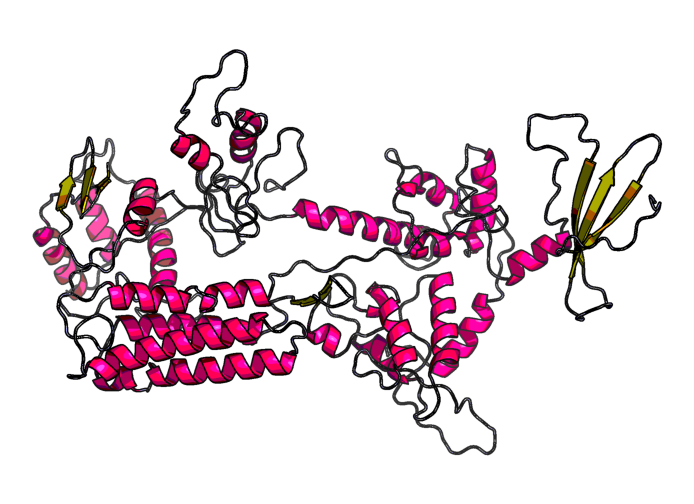
\includegraphics[width=0.6\textwidth]{psd1_struct.png}
    \caption[Predicted Structure of Pds1]{RaptorX Predicted Structure of \textit{P. tetaurelia}
    Pds1 protein (PTETP600032001). No functional annotations could be made using this structure.}
    \label{fig:pds1_struct}
\end{figure}

\subsubsection{Cid}

Two Cid orthologues were identified in each \textit{P. bursaria}
transcriptome.  Additionally, a closely related Cid3 orthologue
was identified in the other \textit{Paramecium} sequences.

Phylogenetic analysis (\cref{fig:cidphlyo}) showed an unclear
picture with both the Yad1g Cid peptides and 1 of the SW1 peptides
branching with moderate support (\(86.7\%\) bootstraps and
a PP of \(0.69\)) within a 
clade composed of Cid1 and Cid3.  Unfortunately, there was
poor support (\(59.1\%\)/\(0.54\)) for the \textit{P. bursaria}
sequences forming a sister to these clades therefore,
their exact placement is unclear.
Additionally, the other
SW1 orthologue branched as the outgroup to all remaining Cid
with high support (\(100\%\)/\(1.00\)). 

This suggests that the orthologues present in Yad1g and one of
the orthologues in SW1 may be the unduplicated ancestor
to Cid1 and Cid3 (named Cid1-3 for convenience).


In general this phylogeny is consistent with a scenario in which a
single ancestral Cid has undergone duplication resulting
in Cid2 and a Cid1-3 ancestor either before
or after the branching of \textit{P. bursaria}.
If this divergence occurred before this speciation
then Cid2 has been lost in \textit{P. bursaria}.
Regardless, there is a clear subsequent 
duplication and divergence of the Cid1-3 ancestor into the modern 
Cid1 and Cid3 
between the \textit{P. bursaria} and \textit{P. caudatum} branches.

Interestingly, the timing location of these events and the presence of 
all 3 Cid homologues in
\textit{P. caudatum} (which shares the single ancient WGD with \textit{P. bursaria})
suggests that this pattern is not
directly related to the polarised position of WGD in \textit{Paramecium}.  

\begin{figure}
    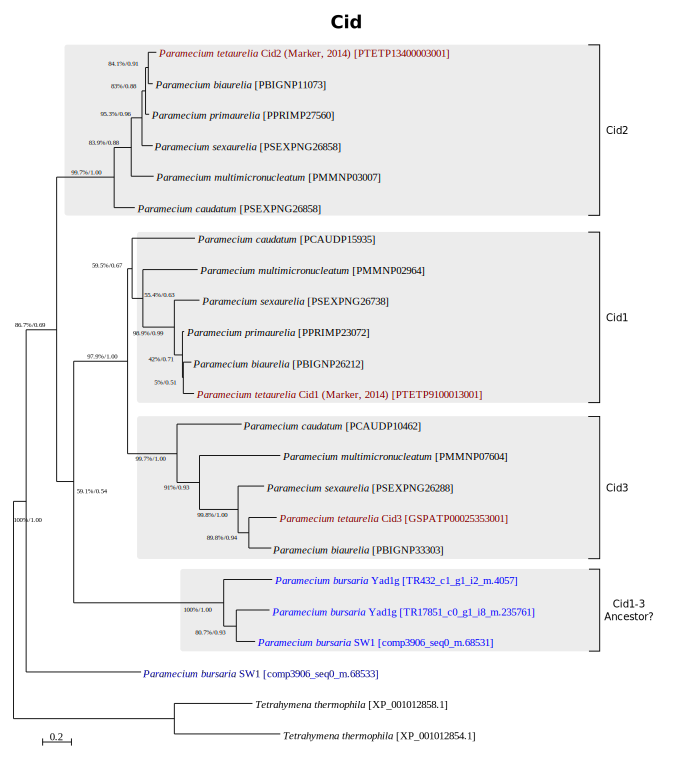
\includegraphics[width=\textwidth]{Cid.pdf}
    \caption[Cid Phylogeny]{
        Phylogeny of Cid1, Cid2, and Cid3 (268 sites) inferred
        using RAxML with rtREV+G and 1000 non-rapid bootstraps.
        Bayesian PP were inferred using MrBayes (2,500,000 generations 
        with 2 runs of 4 chains and a 10\% burn-in).  Phylogeny
        shows a potential orthologue of an ancestral pre-divergence
        version of Cid1 and Cid3 (named Cid1-3) in \textit{P. bursaria}
        Yad1g and SW1 and an uncertain Cid orthologue possibly
        related to Cid2 depending on timing of the Cid1-3 and Cid2 divergence
        in \textit{P. bursaria} SW1.}
    \label{fig:cidphlyo}
\end{figure}

\subsubsection{Rdr}

Two putative sequences were identified by Rdr1 and Rdr2 searches in each
\textit{P. bursaria}.  Phylogenies of these sequences (\cref{fig:rdr12_phylo})
indicate that \textit{P. bursaria} has an orthologue of
Rdr2 (strong support (\(99.9\%\)/\(1.00\)) of an outgroup to the Rdr2 sequences).
The other sequences from both transcriptomes branch basally
to the other \textit{Paramecium} RdRPs with moderate/weak support
and may nor may not be an orthologue of Rdr1.

\begin{figure}
    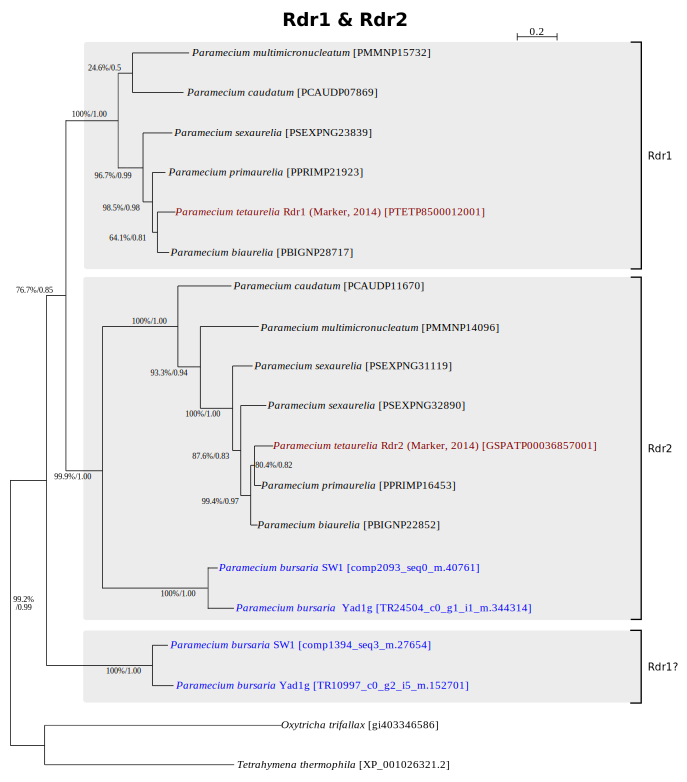
\includegraphics[width=\textwidth]{Rdr1_2.pdf}
    \caption[Rdr1 and Rdr2 Phylogeny]{Phylogeny of Rdr1 and Rdr2
        (691 sites) inferred using RAxML with LG+G+F and 1000
        non-rapid bootstraps.  Bayesian PP were inferred using MrBayes
        (2,000,000 generations with 2 runs of 4 chains and a 5\% burn-in)
        and annotated onto the RAxML phylogeny. Phylogeny
        shows a homologue of Rdr2 in \textit{P. bursaria} as well
    as a potential ancestral or Rdr1 homologue.}
    \label{fig:rdr12_phylo}
\end{figure}

Rdr3 analysis didn't identify any hits in the \textit{T. thermophila}
or \textit{O. trifallax} outgroups but did find an orthologue
in both \textit{P. bursaria} transcript sets.  These branched
as a sister to the other \textit{Paramecium} with strong support
suggesting that they may be orthologous to the \textit{P. tetaurelia}
Rdr3. The phylogeny recapitulated the taxonomy of the ciliates (\cref{fig:rdr3_phylo}).
However, the lack of homology to the other Rdrs indicates that
this Rdr may have been an independent innovation arising basally to the \textit{Paramecium}
clade and is unrelated to Rdr1 and Rdr2.

\begin{figure}
    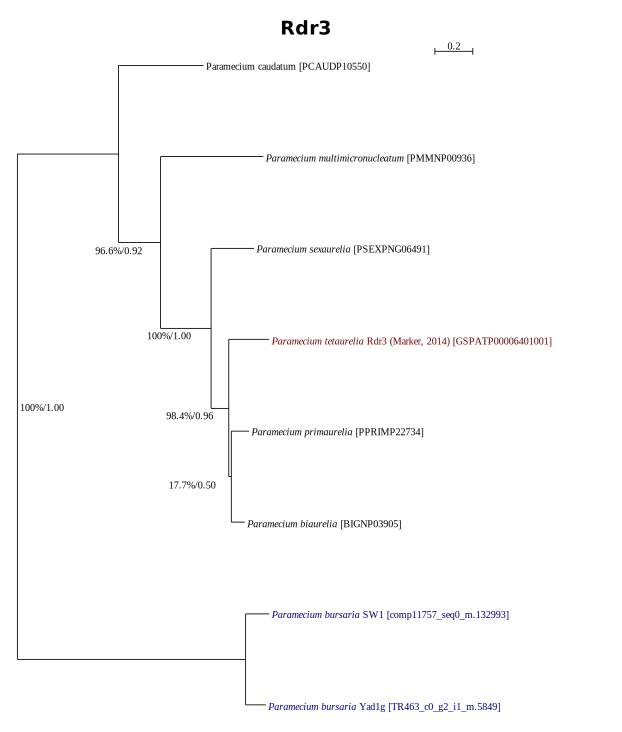
\includegraphics[width=\textwidth]{Rdr3.pdf}
    \caption[Rdr3 Phylogeny]{Phylogeny of Rdr3 (432 sites)
        inferred using RAxML with JTT+G+F and 1000 non-rapid
        bootstraps. Bayesian PP were inferred using MrBayes
        (2,000,000 generations with 2 runs of 4 chains and a 5\% burn-in)
        and annotated onto the RAxML phylogeny.  Phylogeny
        shows the presence of a likely Rdr3 in \textit{P. bursaria}.}
    \label{fig:rdr3_phylo}
\end{figure}

\subsubsection{Piwi}

There were a large number of Piwi detected homologues across
the datasets. Specifically, 16 Piwi in the \textit{P. bursaria} SW-1
transcriptome and 5 in the partial genome, and 17 in the \textit{P. 
bursaria} Yad1g transcriptome.
Due to the large size of this family, large number of paralogues
and relatively short sequences phylogenetic inference
of these sequences proved largely intractable. There are Piwi
homologues present in \textit{P. bursaria} although their exact
relation and function is unknown.


\subsection{dsRNA collisions}

The total number of unique collisions between the endosymbionts and 
the various classes of subject transcriptomes were plotted
(\cref{fig:unique_collisions}). 
This showed next to no collisions with Archaea, moderate levels of total
collisions with Bacteria and generally higher levels of collision
with the Eukaryotes.  The elevated number of collisions with eukaryotic
transcriptomes is not suprising given their 
phylogenetic psoition and gene content.  However, the difference in total 
collisions between archaea and bacteria is potentially interesting. 
It is possible this reflects the sequencing bias in archaea
towards extremophiles which often have compositional adaptations.


Additionally, as might be expected from their close relationship with the 
green algal endosymbionts some of the most frequent collisions were 
with the other green algae.
Interestingly, the three ciliate species displayed a generally low number of collisions 
but there was moderate to high levels of collision against the two
\textit{P. bursaria} host transcriptomes.  This potentially
indicates a higher level of collision between the active host genome 
rather than its total genome.

\begin{figure}
    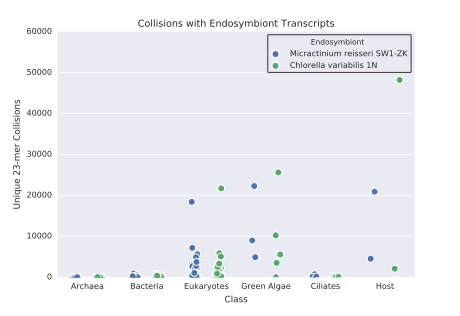
\includegraphics[width=\textwidth]{unique_collisions.pdf}
    \caption[Unique eDicer Collisions by Subject Class]{The number of unique 23-mer
        collisions 
        between transcripts from the \textit{C. variabilis} 1N
    and \textit{M. reisseri} SW1-ZK endosymbionts and different
classes of subject transcripts.  The y-axis is truncated to better
separate the classes however, the the only taxa that had more than 6000
unique collisions were \textit{Coccomyxa variabilis} NC64A and \textit{Chlorella subellipsoidea} C-169
, \textit{Arabidopsis thaliana}, \textit{Chlamydomonas reinhardtii} and transcripts
from the two host bins \textit{P. bursaria} SW1 and \textit{P. bursaria} Yad1g.  
This suggests RNAi-cross talk could be occurring between the host and endosymbiont
and would likely occur at higher rates than occurs between \textit{Paramecium}
and their bacterial prey.}
\label{fig:unique_collisions}
\end{figure}

The collision level was relatively consistent for both endosymbionts
when compared to the same subject (\cref{fig:consistency_most}). 
However, there are visibile exceptions where a given subject
transcriptome has far more collisions against one of two
endosymbiont transcripts than the other.  This can be seen
in the line in the pairplots with sharp angles instead of
being close to level. 

\begin{figure}
    \centering
    
\includegraphics[width=\textwidth]{consistency_unique_coll.pdf}
    \caption[Pair-plot of Normalised Collisions in Both Endosymbiont]
    {Pair-plot of the normalised collisions in Archaea, Bacteria
    and Eukaryotes showing the relative consistency of the
number of hits between the two endosymbionts.  Lines join the number
of collisions to the same subject transcriptome in the different
endosymbiont transcriptomes.  Colour is merely for illustration
purposes and has no significant meaning.
The plot shows that overall the collisions are relatively consistent but there
are aberrations where one endosymbiont has far more collisions
to a given subject than the other.}
    \label{fig:consistency_most}
\end{figure}

This is particularly obvious in 
the comparison of collisions between the host endosymbiont pairs
(\cref{fig:pairs_endo}).  There is a considerable difference
in collisions for the \textit{C. variabilis} 1N endosymbiont
from the Yad1g1N culture with next to no collisions
against the \textit{P. bursaria} from the other culture
but a high level of collisions against its own host.
Interestingly, \textit{M. reisseri} was relatively
consistent across both hosts with only slightly more
hits to its own host. 
This suggests a potential problem
in the binning of endosymbiont and host transcripts, especially
in the \textit{P. bursaria}-\textit{C. variabilis} Yad1g1N transcriptome.

\begin{figure}
    \centering
    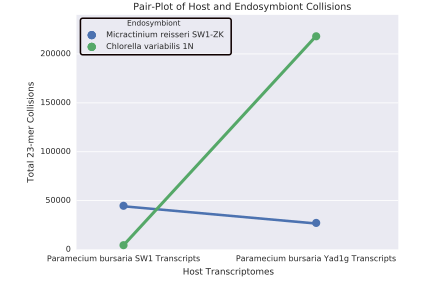
\includegraphics[width=0.7\textwidth]{host_endosymbiont_collisions.pdf}
    \caption[Pair-plot of Collisions in Host-Endosymbiont pairs]
    {Pair-plot of the total number of collisions between
        the two endosymbiont transcriptome sets and 
        the two host transcriptome sets. \textit{M. reisseri}
        has a relatively consistent number of collisions
        against both hosts, however, the \textit{C. variabilis}
        transcriptome has a significantly higher number
        of collisions against it's own endosymbiont.
        This suggests potential issues with the binning
    of transcripts in the Yad1g1N transcriptome.}
    \label{fig:pairs_endo}
\end{figure}


In order to test to what degree the number of collisions was related
to the length of the subject query, a simple linear regression
was conducted (\cref{fig:edicer_collisions_by_length}).  
This demonstrates there is at least a partial linear dependence between the 
length of the query and the number of collisions as would be expected.

\begin{figure}
    \centering
    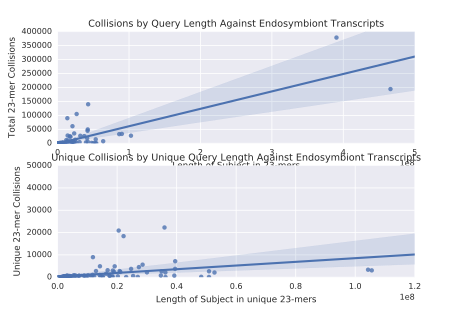
\includegraphics[width=\textwidth]{length_collisions_regs.pdf}
    \caption[Regression of eDicer Collisions by Query Length]{Linear Regressions
    of the relationship between the number of collisions as query length
increases. Features points from collisions with both \textit{C. variabilis} 1N
and \textit{M. reissier} SW1-ZK.  Dark blue cloud indicates \(95\%\) confidence
intervals.  
The top plot shows total collisions against
total length whereas the bottom analysis only looks at unique collisions
against unique length so theoretically ameliorates the effect of repetitative 
transcripts/many isoforms.  Both show a clear if noisy (correlation coefficients
of \(0.18085\) and \(0.02811\) respectively) linear relationship and thus
support that the size of a transcriptome plays a role in the number of collisions.}
    \label{fig:edicer_collisions_by_length}
\end{figure}

Normalising the unique number of collisions by the unique length of
the subject predicted transcriptome led to some interesting results (\cref{fig:edicer_unique_norm})
Collisions with Eukaryotes largely were reduced to being on-par
with collisions against Bacteria.
Despite collisions against the ciliates relatively disappearing,
there was still considerable levels of potential RNAi cross-talk against
the host transcriptomes and green algae.

\begin{figure}
    \centering
    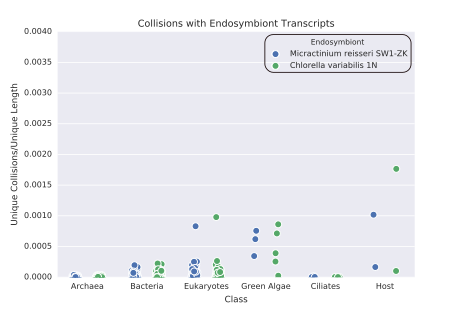
\includegraphics[width=\textwidth]{unique_norm_collisions.pdf}
    \caption[Normalised Unique eDicer Collisions]{The number of collisions
        between transcripts from the \textit{C. variabilis} 1N
    and \textit{M. reisseri} SW1-ZK endosymbionts and different
classes of subject transcripts normalised by the unique length of those
subjects.}
    \label{fig:edicer_unique_norm}
\end{figure}

\section{Discussion}

\subsection{No dsRNA RNAi inducible phenotypes in \textit{P. bursaria} SW1}

Despite numerous attempts, all feeding experiments failed to induce
any of the RNAi knockout phenotypes.  RT-PCR tests (not shown) with the Bug22
and BBS7 constructs demonstrated
that the \textit{E. coli} was successfully transformed and could 
inducibly express the dsRNA.  
This indicates that dsRNA is either incapable of escaping the digestive vacuole
or that \textit{P. bursaria} does not have an active pathway for exogenous dsRNA 
induced RNAi.

The potential failure of microinjection of dsRNA directly into the MAC
to elicit RNAi phenotypes would support the absence
of an active dsRNA induced RNAi pathway. 
However, the high methodological difficulty involved in identifying and injecting
the MAC without lysing the cell (\cref{fig:microinjection_nucleus}) 
means microinjection may have only failed to induce RNAi due to failure
to correctly microinject \textit{P. bursaria}.   \textit{P. bursaria}
was particularly prone to lysis relative to \textit{P. tetaurelia} and
there were greater issues with trichocysts blocking the microinjector. 
Attempts made to inject GFP into the MAC also failed to generate fluorescence
localised to the MAC.  This indicates that the failure of microinjection is
primarily technical and cannot be used to make inferences about the state
of the RNAi pathway in host. 

\begin{figure}
    \centering
    \includegraphics[width=0.7\textwidth]{microinjection_hard.pdf}
    \caption[DAPI Stained \textit{P. bursaria} MAC]{
        DAPI stained \textit{P. bursaria}
        MAC to demonstrating how difficult it is to accurately identify the limits
        of the MAC for microinjection.  Top left panel shows 3 \textit{P. bursaria}
    cells under light microscopy as they appear when attempting
microinjection. Top right shows fluorescence from DAPI staining to demonstrate
where the MAC nuclei are location.  Bottom panel is an artificial overlay
of the light microscopy and DAPI staining.}
    \label{fig:microinjection_nucleus}
\end{figure}

Unforunately, the alternative transgene RNAi methodology \citep{Galvani2001} 
(which was not attempted) also involves microinjection of the MAC with
the transgene construct itself.  Therefore, even if the transgene
pathway is present and active it may still not be possible to reliably
induce RNAi in \textit{P. bursaria}.

\subsection{Missing components of RNAi pathway in \textit{P. bursaria}}

An investigation into the RNAi pathway components identified by \citep{Marker2014}
revealed the absence of one required component for the exogenous dsRNA
pathway (Pds1) and depending on the function of a putative ancestral
Cid protein the absence of a factor in the common pathway or another
exogenous dsRNA pathway (\cref{fig:rnai_summary}).


Pds1 is totally absent outside of the post-\textit{P. bursaria} 
\textit{Paramecium} clade.
A phylogenetic analysis of Pds1 sequences (\cref{fig:pds1}) 
recapitulated the established 
\textit{Paramecium} taxonomy (\cref{fig:paramecium_genomes}).
This suggests that Pds1 was either acquired after the divergence of \textit{P. bursaria}
and \textit{P. caudatum} or was lost in \textit{P. bursaria}.
The pattern of paralogues would more likely support the former scenario.
The lack of paralogues (with the exception of a terminally duplicated \textit{P. multimicronucleatum}
copy) in the \textit{P. aurelia} complex species is interesting.  As the presence
of Pds1 in \textit{P. caudatum} indicates that this should have undergone
duplication during the two subsequent WGD events.  Potentially, this represents
serial losses in these species.

It is possible that Pds1 is present and just hasn't been recovered 
in the partial transcriptomes because it is not being transcribed (or is 
transcribed at a very low level) during endosymbiosis.  It is also
possible it is missing in the partial genome due to the incompleteness
of this data.  However, the combination of being missing in all 3 datasets
as well as any non-\textit{Paramecium} ciliates indicates that
it is likely not present in \textit{P. bursaria}.

\begin{figure}
    \centering
    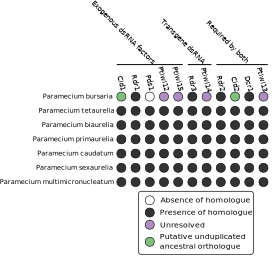
\includegraphics[width=0.8\textwidth]{RNAi_factors_summary_figure.pdf}
    \caption[Summary of RNAi Factors in \textit{Paramecium} species]{Coulson plot
        showing the absence/presence of RNAi pathway factors
    identified in \textit{P. tetaurelia} \citep{Marker2014} across the \textit{Paramecium}
clade.}
    \label{fig:rnai_summary}
\end{figure}

The Cid proteins are difficult to resolve, either \textit{P. bursaria}
has an undiverged ancestral version of the Cid proteins or has a
Cid1-3 ancestor and has secondarily lost Cid2.
This depends on the timing of the Cid2 and Cid1-3 divergence, if
it occurred after the branching of \textit{P. bursaria} from the rest
of the clade then the latter scenario is more likely and vice versa.

If the latter scenario is true then Cid2 has been lost 
and if the \textit{P. bursaria} RNAi
pathways require the same components as \textit{P. tetaurelia} this may
mean both the transgene and dsRNA pathways might not be active. 
Additionally, if the Cid1-3 ancestor or the ancestral undiverged
Cid does not have function of \textit{P. tetaurelia}'s Cid1 then
the exogenous dsRNA pathway may not be active in \textit{P. bursaria}.


\begin{figure}
    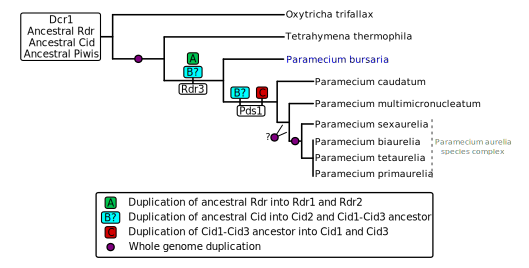
\includegraphics[width=\textwidth]{RNAi_factor_evolution_summary.pdf}
    \caption[Summary of RNAi Factors Evolutionary Scenarios in \textit{Paramecium} species]{
        Diagram showing the \textit{Paramecium} clade with \textit{Tetrahymena} outgroup 
        showing the putative evolutionary scenarios behind the currently
        observed distributed of RNAi factors.
    }
    \label{fig:rnai_evol_summary}
\end{figure}

The unresolved Piwis also represent potential issues with the RNAi pathway
but the only way to thoroughly investigate the roles of these proteins would
be targeted mutagenic screening or a similar approach.

The low levels of sequence homology suggests independent innovation 
of Rdr3 and potentially sheds doubt on its relationship to the ancestral
Rdr that this analysis confirms was likely present in 
was present in the first WGD \citep{Marker2014}.


Interestingly, the general disposition of paralogues across the \textit{Paramecium}
clade does not recapitulate the three established WGD events in this group.
For example, there is a relatively consistent number of paralogues of 
all components, especially RdRPs and Cid proteins in \textit{P. caudatum} 
despite this clade having undergone the same number of WGD as \textit{P. bursaria}
and not sharing the 2 recent WGD with the majority of the remaining \textit{Paramecium} 


\subsection{Endosymbiont ``collision'' hypothesis}

Hypothetically \textit{Paramecium bursaria}
may have deactivated/lost feeding induced RNAi (specifically the
uptake of RNA from vacuoles) as a consequence
of the greater levels of potentially deleterious cross-talk between
it and its eukaryotic green algal endosymbionts.  
As an exogenous RNAi response is not essential 
for viability in \textit{P. tetaurelia} \citep{Marker2014} loss
of this system in \textit{P. bursaria} may not have a high fitness cost.


On first glance the high levels of collisions between endosymbiont
transcripts against host and eukaryote classes in general support this
hypothesis (\cref{fig:unique_collisions}).
However, there were low levels of collisions between endosymbiont transcripts
and ciliate transcripts indicating that the collision levels
observed between host and endosymbiont require an additional explanation.
The first scenario is that the active host transcriptome during
endosymbiosis is not representative of all possible host transcripts
and features a much higher level of collision with the endosymbiont.
The second scenario is that the levels of collisions between host and
endosymbiont actually reflects misbinning of endosymbiont transcripts
as belonging to the host.  A comparison of the collisions
of each endosymbiont against its own host and the other host \textit{P. bursaria}
(\cref{fig:pairs_endo}) suggests that binning error may explain
some of this difference and that the binning the Yad1g1N transcriptome
has potentially more issues than the SW1-ZK (CCAP 1660/12) transcriptome.
This might be explained by the fact that only half the sequenced
libraries in Yad1g1N actually contained the \textit{C. variabilis} 1N endosymbiont
as this dataset originated from an an analysis of transcriptomic
profiling of \textit{P. bursaria} with and without its endosymbiont \citep{Kodama2014}.


There is a linear relationship between the unique size of a transcriptome
in terms of 23-mers and the number of collisions (\cref{fig:edicer_collisions_by_length}).  
This is expected
as a longer set has a higher probability of a random match by chance.
When the number of collisions is normalised by the length of the subject (\cref{fig:edicer_unique_norm})
the level of collisions from eukaryotes is largely on-par with
those of bacteria.  However, as eukaryotes have larger genomes
the un-normalised number of collisions is more reflective of biological
reality.  Indeed, the size and diversity of their transcriptome
may be the reason why eukaryotic cross-talk is potentially
more problematic than that of bacterial cross-talk.


It might be interesting to test the linear relationship between phylogenetic
relatedness and the number of K-mer collisions.  For example, phylogentic distances
between the endosymbiont and various taxa could be derived from an established
published multi-gene analysis that includes these species and regression
conducted using this as a feature. 

One down-side of the efficient K-mer hashing based ``eDicer'' design is that
it only finds exact matches.  RNAi has been found to not always require exact
sequence matches to induce knock-down \citep{Elbashir2001} therefore,
this analysis potentially misses a large amount of near-identical collisions.
Fortunately, it is probably a relatively safe assumption that the number
of identical collisions correlates strongly with the number of near-identical collisions.

Finally, while this may not have thoroughly resolved the question of matches
eDicer may form a useful tool in the rapid screening of off-target effects
in the RNAi analyses in different organisms.   It is considerably
more efficient than than cutting and alignment based methods such as that
offered on ParameciumDB \citep{Arnaiz2011}.

\section{Conclusions}

RNAi induced phenotypes could not be created in \textit{P. bursaria} SW1 from CCAP1660/12
via feeding experiments.  The absence of Pds1 in \textit{P. bursaria} offers a potential 
explanation for this as this protein has been implicated in playing some undefined role
in the uptake of RNA (dsRNA or ssRNA) from digestive vacuoles \citep{Carradec2015}.
As ``eDicer'' identified that there are a large number of 23-mer collisions
between \textit{P. bursaria} transcripts and eukaryotic transcriptomes (especially
the green algal endosymbionts) the loss/deactivation of the uptake of RNA from 
digestive (or potentially perialgal) vacuoles could be a consequence of 
a eukaryotic endosymbiont in \textit{P. bursaria}.  
The relatively lower levels of RNAi cross-talk between
\textit{Paramecium} and bacterial endosymbionts and/or food species may prove
less deleterious than eukaryotic cross-talk. 

Due to Pds1 only likely being involved in uptake from a food vacuole it is possible
that dsRNA could still be induced by direct microinjection.  Similarly, 
microinjection of transgenes may still be possible.  Unfortunately, microinjection
has proven difficult technically in \textit{P. bursaria}.  Further optimisation
of the experimental method and training is required to thoroughly test
the activation or deactivation of injected dsRNA or transgenes.

Alternatively, the potential ancestry of the Cid proteins in \textit{P. bursaria}
may indicate a deactivation/absence
of RNAi by the pathways identified by \citep{Marker2014} in \textit{P. bursaria}
depending on the relative functionality of this ancestral form.
Further analysis of RNAi systems in \textit{P. bursaria} and other \textit{Paramecium}
species would be required to further answer this question.

